While we are limiting our infinite matter calculations only to pure neutron matter ($x_p = 0.0$) and symmetric nuclear matter ($x_p = 0.5$), we can still calculate a quantity that is important to studies of infinite nuclear matter and the nuclear equation of state. The quantity is the symmetry energy which is defined as:

    \begin{equation}
        \mathcal{l}(\rho) = E(\rho, x_p=0) - E(\rho, x_p=1/2).
    \end{equation}

Fig. \ref{fig:symmetry} shows the symmetry energies calculated for both the CCD approximation (red) and the CCD(T) approximation (blue) for densities around nuclear density. Additionally, the symmetry energies calculated with full converged energies at M = 1,478 for PNM and M = 2,956 for SNM are shown with the solid lines, and the symmetry energies calculated with SRE predictions are shown with triangular markers. Additionally, the uncertainty on the SRE predictions is shown with error bars. This uncertainty comes from the Gaussian process algorithm.  Note that this plot is energy per nucleon instead of correlation energy per nucleon as the other plots in this chapter.

\begin{figure}
    \centering
    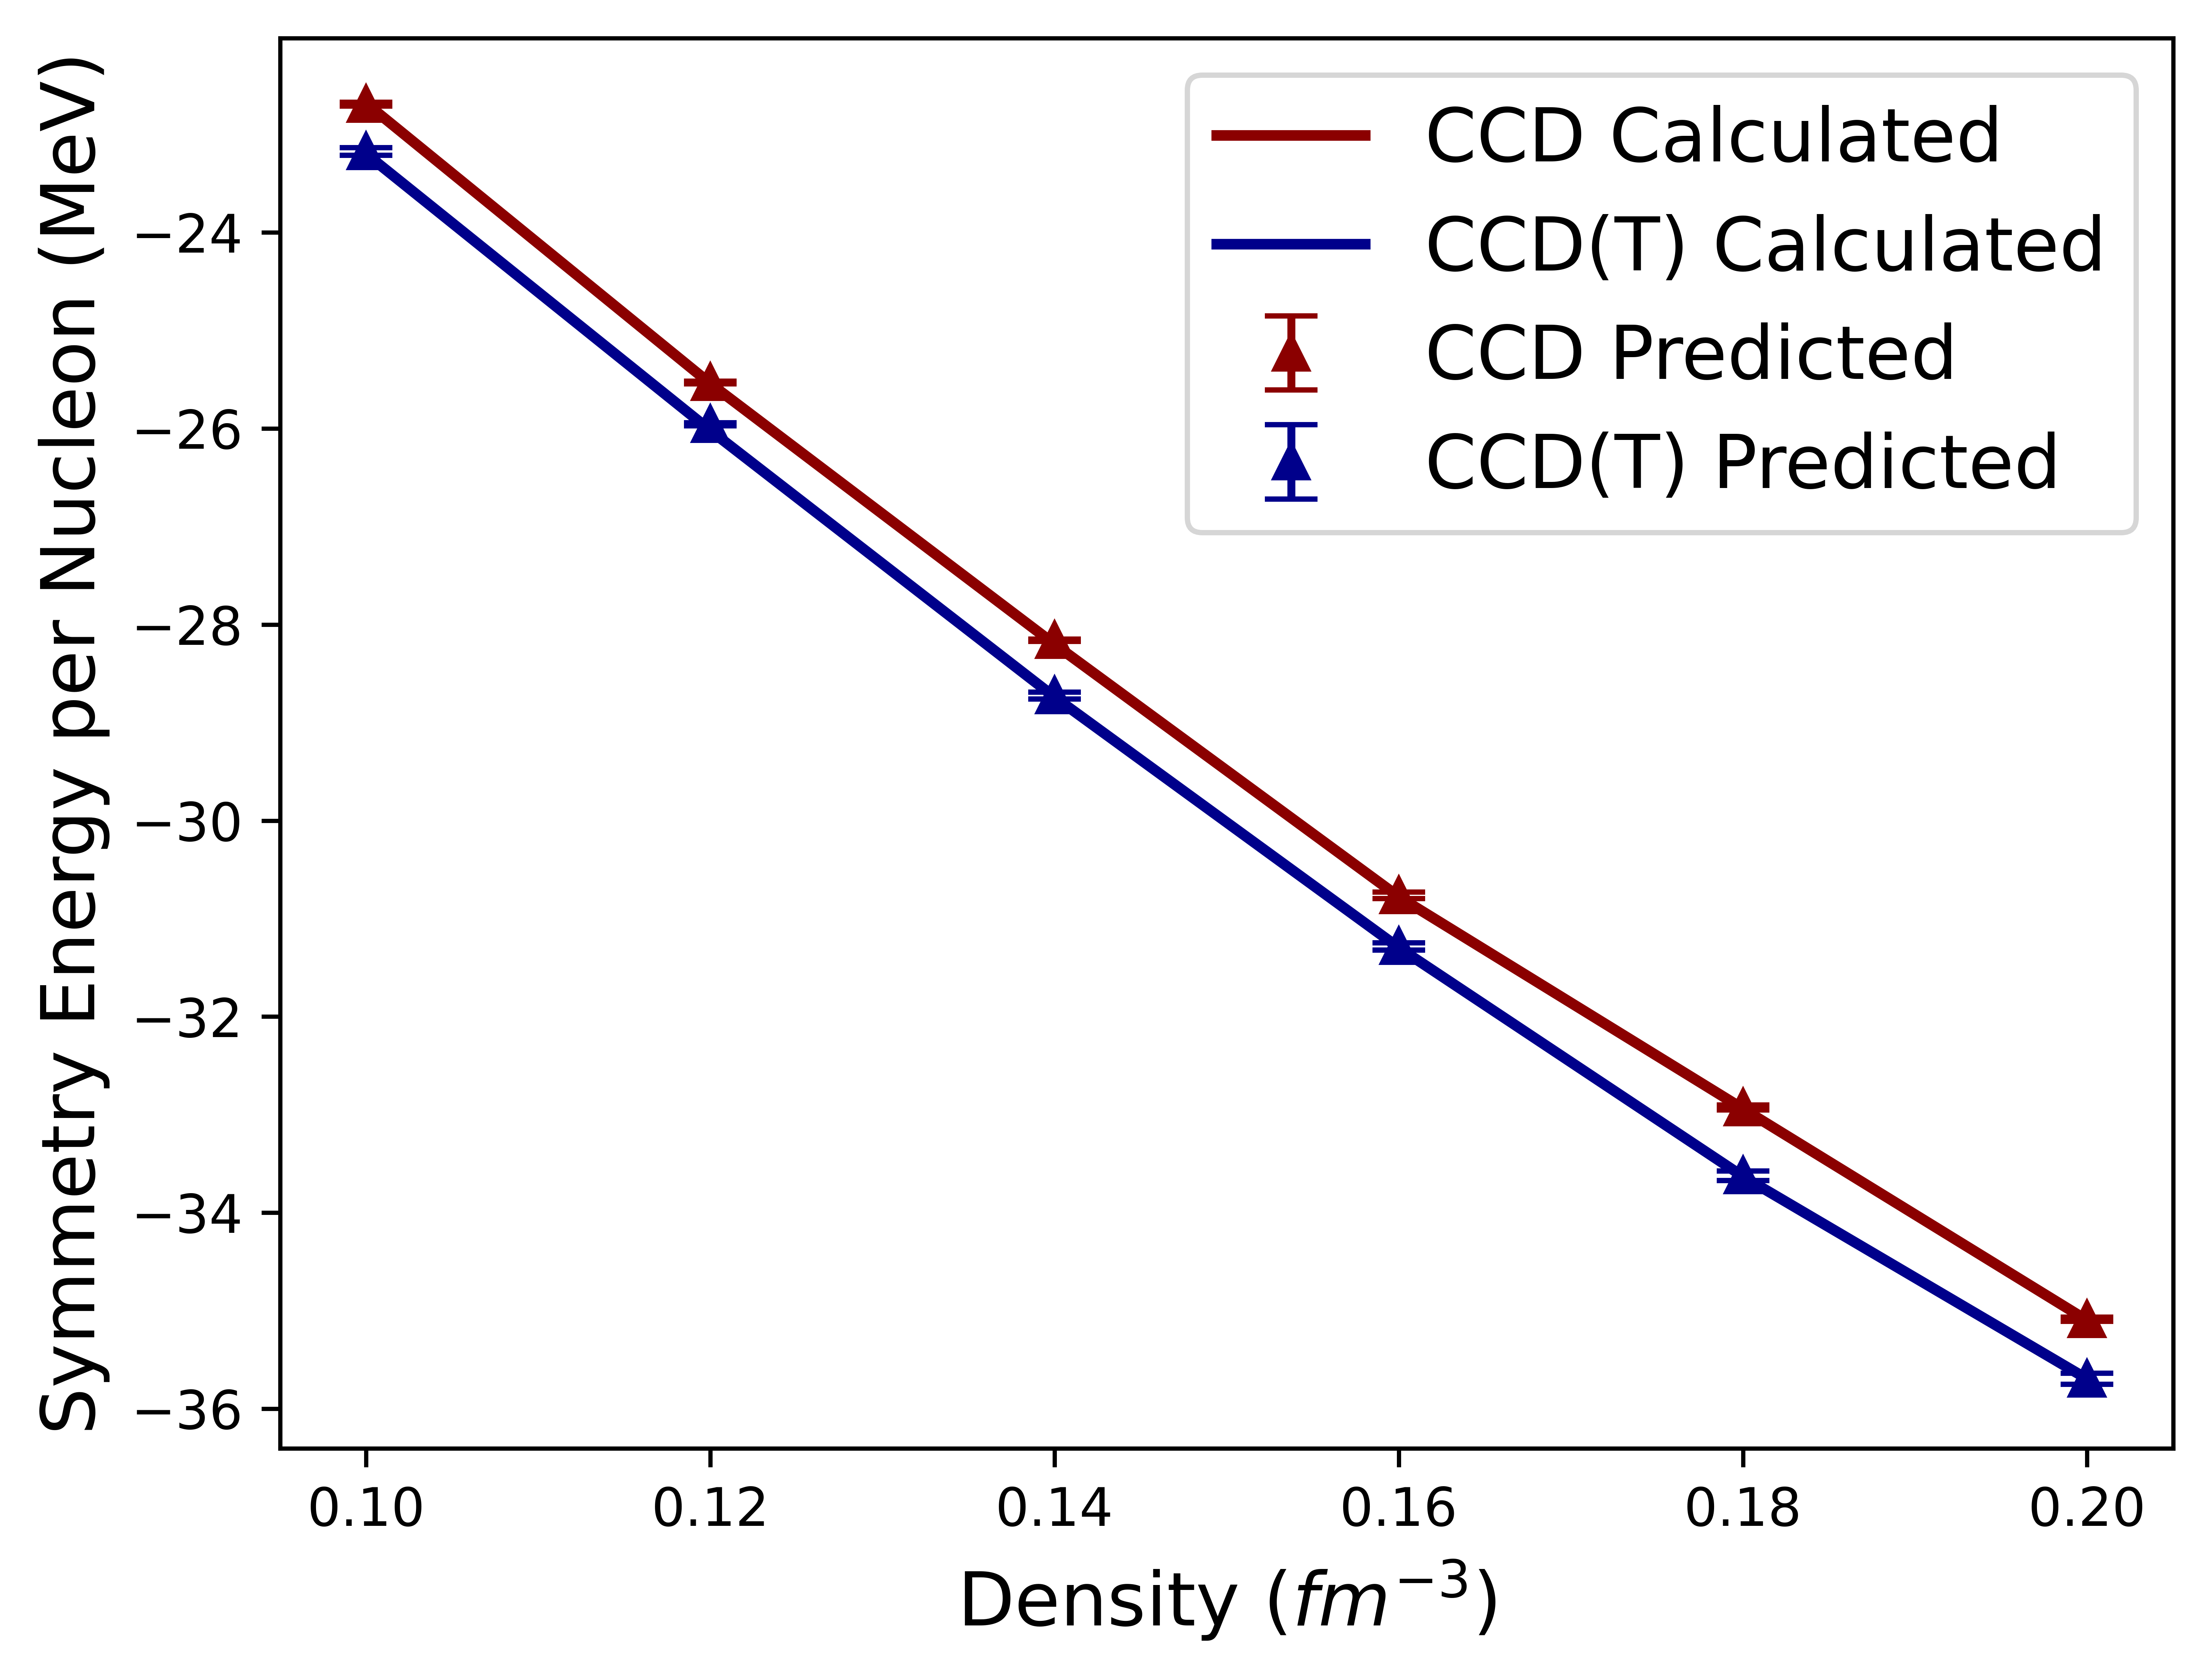
\includegraphics[scale=0.75]{Images/Chapter8/symmetryenergy.png}
    \caption{The symmetry energy for infinite nuclear matter is calculated using the CCD approximation (red) and the CCD(T) approximation (blue). The symmetry energy calculated from fully converged calculations is shown with the solid lines and SRE predictions with the triangular points. Error bars also represent the uncertainty on the symmetry energy from SRE predictions from the Gaussian process algorithm.}
    \label{fig:symmetry}
\end{figure}

For the CCD approximation, the average percent error between the two data sets is 0.056$\%$, and for the CCD(T) approximation, it is 0.078$\%$. Note that these percent errors are much smaller than previous results because we are considering the total energy instead of just the correlation energies so small differences have much less of an impact. We also need to consider time savings as a justification for performing the SRE method over the complete calculations for the symmetry energy. The time needed to generate all 12 points (6 for PNM and 6 for SNM) needed to calculate the symmetry energy at M = 1,478, or 2,956, is 661.22 node hours for the CCD approximation and 2608.11 node hours for the CCD(T) approximation. The time needed to generate all training data for the CCD approximation is 353.05 node hours and 1472.10 node hours for the CCD(T) approximation. The training data requires just 55.8$\%$ of the computational time it takes to generate the fully converged energies and most of this time is due to the high cost of SNM calculations. This leads to a time savings of 20.11 \textit{node days} for the CCD approximation with an average error of 0.056$\%$. The time savings for the CCD(T) approximation is 47.33 \textit{node days} with an average percent error of only 0.078$\%$. Therefore, when calculating the symmetry energy, the SRE method provides an accurate prediction and can save many days of computational time.